% !Mode:: "TeX:UTF-8"
%%% Local Variables:
%%% mode: latex
%%% TeX-master: t
%%% End:

\chapter{引言}
\label{chapter:introduction}

\section{研究背景}

短波通信又称高频通信~\cite{胡中豫2003现代短波通信},是指使用频率范围在高频(HF)的无线电进行通信的方式~\cite{董彬虹2007短波通信的现状及发展趋势}。短波通信主要利用天波电离层反射,所以无需中继站即可实现远距离通信,具有机动性强、设备成本低、对基础设施依赖小的优点,因此被广泛应用于广播、军事和抢险救灾等领域。

而同时,短波通信的缺陷也非常突出,因为受电离层变化和多径传播等因素的影响,短波通信的信道非常不稳定,导致其通信质量起伏较大,影响通信的稳定性。应对这一问题,军事中应用短波语音进行地空通信时,目前有一种解决方案:如图~\ref{fig:sys_struct}所示,在地面不同地点建立多个短波信号接收基站,接收来自空中飞机的短波语音。再将这多路信号汇总到一起,由人工选择一路质量最优的信号接入给地面指挥人员。人工选择需要的人工成本高,且稳定性和可靠性都不高,亟待使用算法代替人工。本文旨在通过对一系列算法及系统的研究,使用算法替代该方案中的人工选择步骤。

\begin{figure}
\centering
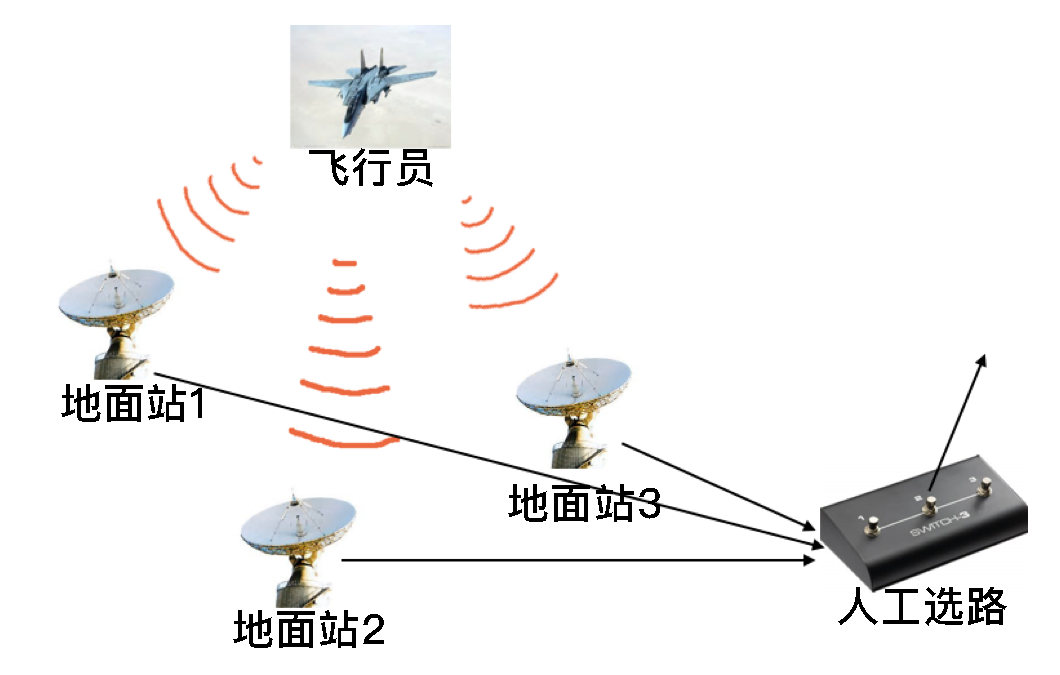
\includegraphics[width=0.8\textwidth]{sys_struct}
\caption{军事应用中的一种地空短波通信系统\label{fig:sys_struct}}
\end{figure}

\section{研究现状}

\subsection{短波通信系统研究现状}

短波通信最早出现于20世纪初,由于其无需借助中继设备即可实现远距离通信的特性,直到今日依然被广泛应用于各个领域,尤其在军事领域短波通信起到了不可替代的最低通信保障作用。在这期间,为了弥补短波通信的不稳定性等劣势,各种技术层出不穷,尤其从20世纪80年代以来,短波通信技术得到了长足的发展。相关技术有自适应选频与信道建立技术、自适应传输速率技术~\cite{clarke2003multilevel}、自适应天线技术~\cite{cook2012adaptive}、高速调制解调技术~\cite{nilsson1997wideband}、抗干扰技术~\cite{andersson1995performance}~\cite{zander1995adaptive}和组网技术等。

与本文比较相关的主要是自适应选频与信道建立技术。

Harmon等人~\cite{harmon1982adaptive}设计了一种可以自动选择最优通信频率的短波通信系统,其基本思想是将测量到的到各个通信站使用各频率信道的信噪比保存在一个矩阵中,持续维持此矩阵,对没有得到更新的信噪比数据随时间进行衰减,然后在发起通信时根据目标通信站自动选择最优的频率进行通信。McRae等人~\cite{mcrae1989frequency}提出的系统同样也是针对多个短波通信站通信时的频率选择问题,其采用的方法是要发送信号的通信站先发送一系列的探测信号,等待接收站的回复来选择最优的通信频率。

自适应选频其实是在频率维度的多路接收以选择最佳信道,而本文的应用场景则是在空间纬度多路接收再自动选择最佳信道。本文的方法是在应用层之上对信道进行评价,即对接收语音的质量进行评价,从而既可以应用于模拟通信也可以应用于数字信号通信,还可以用在自适应选频上。

\subsection{语音质量评价研究现状}

随着各类语音通信技术、语音编码、存储、增强等系统的发展,对语音质量的评价问题显得越来越重要。好的语音质量评价方法是评估这些系统的基础,有时也是改进系统的重要途径。语音质量评价从主体上分类可分为主观评价和客观评价两大类。

主观评价是指由人的主观感受来进行评价,客观评价则是通过算法分析语音的不同特性、比较接收语音和原始语音等,对语音进行评价~\cite{肖累累2013语音质量客观评价方法的研究}~\cite{moller2011speech}。

主观评价可以按照ITU-T Recommendation P.800~\cite{rec1996p}中的ACR评分方法得到语音的主观平均意见分(MOS)。在规定的环境下,让志愿者试听各个语音并按照质量给语音分类打分,分值为1至5分的整数分值。再计算所有志愿者评分的均值即可得到语音的主观平均意见分(MOS)。

主观评价能够最真实地反映人的主观感受,但是需要投入大量人力,耗费很多时间和经费,而客观评价则可以快速、自动地给出评分,客观评价算法的目标是尽量真实的反映人的主观感受,故而评价客观评分算法的优劣一般通过比较其结果和主观评价结果的相关性。

客观评价方法可以分为单端算法和双端算法两类,双端算法是指需要有原始纯净语音信号作为参考的算法,而单端算法则是指仅根据输出或接收语音进行评价的算法。

双端算法的想法很简单——通过比较输出或接收到的语音与原始语音的感知上的差异来评价语音质量,这类的算法模型包括Perceptual Evaluation of Speech Quality(PESQ)~\cite{recommendation2001perceptual},Perceptual Objective Listening Quality Assessment(POLQA)~\cite{rec2011p}等。PESQ~\cite{recommendation2001perceptual}对输入输出的语音先做电平变换到同样等级,经过一个模拟听筒的滤波器,在时间上对齐之后,再模拟人的听觉系统进行一个变换,然后提取出两个参数衡量信号的畸变大小,最后在时间和频率上聚合参数给出语音的最终评分。POLQA~\cite{rec2011p}是在PESQ基础上的改进,一是使用了更复杂的时间上的对齐机制,使之可以适应更复杂的时间方向的畸变,二是在评价模型上针对宽带、超宽带的语音信号做了优化。

单端算法面向的问题是没有原始语音作为参考的,在这种情况下,一种思路是通过一些先验知识来推测原始语音信号和信号变差的程度,从而对语音质量进行评价。例如Gray P等人~\cite{gray2000non}以及Malfait等人~\cite{malfait2006p}利用语音的产生模型来反推原始语音信号,进而评价语音质量。后者的算法P.563被国际电联电信标准化部门(ITU-T)收录为推荐算法。Falk等人~\cite{falk2006nonintrusive}使用高斯混合模型(GMM)来拟合从语音中提取的特征因子的概率分布,使用干净的语音训练学习模型,然后对畸变带噪语音做评分。Kim等人~\cite{kim2007anique+}提出的ANIQUE+算法则是基于人耳对语音的感知模型,提取语音的时域包络信息进而进行评分。该算法被美国国家标准学会(ANSI)收录。

另一种思路则是从输出语音中提取一些特征,然后根据这些特征来进行评分。例如Grancharov V等人~\cite{grancharov2006low}提出的LCQA算法,对每一帧语音提取11维向量特征,再全局统计特征,输入到高斯混合模型映射为最终的评分。Narwaria M等人~\cite{narwaria2010non}则通过提取语音的梅尔频率倒谱系数(MFCC)特征,再使用支持向量机回归(SVR)来预测语音的质量评分。

近些年随着大数据和机器学习技术越来越成熟,也有不少研究将深度神经网络等机器学习模型应用到其中。例如Patton B等人~\cite{patton2016automos}使用深度递归神经网络来学习语音评分模型,采用两个长短时记忆网络(LSTM)的结构。 Sharma等人~\cite{sharma2016data}通过提取语音的特征之后使用分类和回归树(CART)进行语音的质量评分。

以上这些语音质量客观评价算法都是针对VoIP系统、语音编码系统、语音去噪系统等提出的,其评价的语音信噪比相对于短波信道的语音而言要高出很多。直接应用到低信噪比的短波信道语音,无法得到让人满意的效果。

% \subsection{语音增强研究现状}

\section{研究目标和研究内容}

本文的主要目标在于研究适用于短波通信语音的客观质量评价算法,以及基于此的短波语音自动选路系统,增强短波语音通信的通信质量和稳定性。

本文的研究内容主要包括:
\begin{enumerate}
\item 针对短波语音的特殊性,本文提出了一种基于语谱图噪音模型的客观质量评价算法和一种基于自编码器的客观质量评价算法。并将这两种算法和两种标准的语音质量客观算法做了实验比较。
\item 基于短波语音客观质量评价算法,本文为实际应用场景设计了一种短波语音自动选路系统,并用实验验证了系统的效果。
\item 为了方便对短波语音的研究和实验,设计实现了一个用于辅助短波语音主观质量评价的在线辅助系统。
\end{enumerate}

\section{论文结构和内容概述}

本文剩余部分的结构如下所示:

第2章主要介绍短波语音客观质量评价算法。介绍了两种客观评价算法,一种是基于语谱图噪音模型的算法,另一种是基于人工神经网络自编码器的算法。前者根据短波语音的噪音特征设计,对于短波语音的质量评价效果非常好,但是算法针对性太强,迁移到其他领域的语音信号时,需要重新分析对应的噪音特征;而后者通过自编码器学习纯净语音信号的语谱特征,可以方便地迁移到其他领域。

第3章主要介绍多路短波语音自动选路系统。首先介绍了多路语音时间对齐算法,然后介绍了基于此算法以及第2章介绍的客观评价算法的自动选路系统。

第4张介绍了语音质量在线主观评价辅助系统,首先介绍了系统的功能和使用方法,然后介绍了系统开发和部署环境及运行原理。

第5章介绍了实验的情况。通过两组实验分别验证了第2章所提算法及第3章所提系统的实际效果,在短波语音数据集上对比了本文所提算法与两种标准质量评价算法的表现。

第6章对本文工作进行总结,并对将来可能的研究方向进行展望。

